% ===================================================================================================
%                                                 |                                                 |
%                                                 |                                                 |
% -------------------------------------------- SECTION ---------------------------------------------|
%                                                 |                                                 |
%                                                 |                                                 |
% ===================================================================================================
\section{Energy grand challenges in embodied AI: perspective and research directions}\label{sec:energy_grand_challenges}
Based on the energy expenditure categories introduced in Sec.~\ref{sec:intro}, we have identified three grand energy demand challenges in embodied AI. We discuss them individually in the following, highlighting their implications on future energy consumption.

% SUBSECTION ========================================================================================
\subsection{\textbf{CHALLENGE 1} (C1). Energy for AI infrastructure}
Most state-of-the-art machine learning algorithms depend on significant volumes of data and a vast number of computational iterations to converge to a solution \cite{Strubell2019EnergyAP}. To accelerate the time spent training such models, researchers and companies take advantage of the readily available infrastructure or use several cloud computing services running on data centers. Serving many purposes, data centers have turned into a relevant sink of energy usage.  For instance, in the six years between 2015 and 2021, the worldwide energy use of data centers moved from 200 TWh to an estimated 220-320 TWh\footnote{Data from the International Energy Agency, see \url{https://www.iea.org/reports/data-centres-and-data-transmission-networks}}. Comparatively, only in Germany, the energy consumption of data centers increased from 10 TWh in 2010 to 17 TWh in 2021. At this rate, experts anticipate that data centers in the country will require 28 TWh by 2030 \cite{Hintemann2022Cloudcomputingdrives}. Fig.~\ref{fig:dataCenterEnergy} illustrates the increasing trend in the energy demand from data centers. \textcolor{red}{According to this trend, this demand amounts for about 1\% of the worldwide electricity consumption in 2021.}
%---
\begin{figure}[!t]
	\centering
	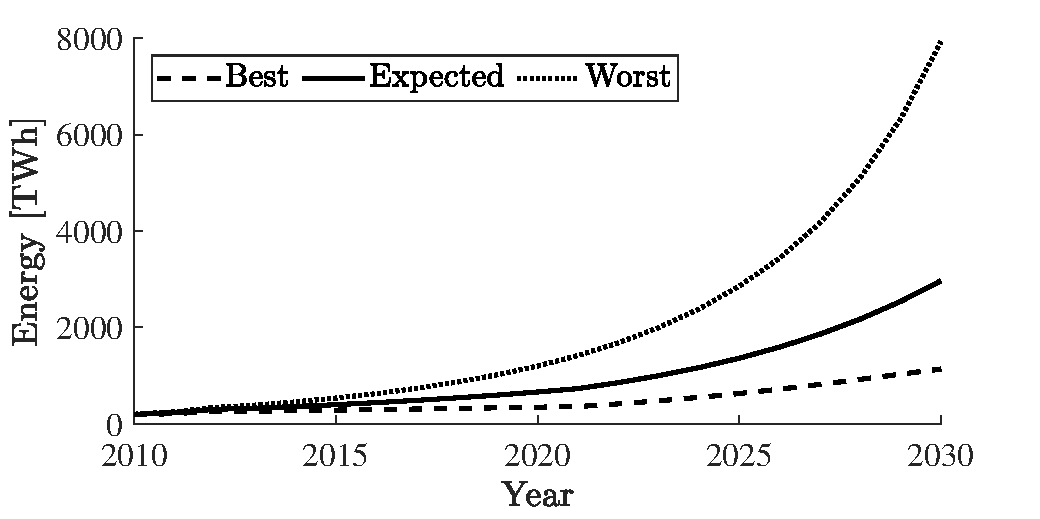
\includegraphics[width=0.9\columnwidth]{fig/data_center_energy_consumption.pdf}
	\caption{Global electricity demand of data centers (adapted from \cite{andrae2015global})}
	\label{fig:dataCenterEnergy}
\end{figure}
% ---
To further exacerbate the problem, unlike reference state-of-the-art machine learning models (e.g., transformer models) that are trained once on a large amount of data. Embodied AI will use models that require constant retraining and re-evaluation, such as neural architecture search \cite{real2019regularized}. A key contribution to increasing the energy consumption of machine learning algorithms emerged because recent techniques allowed data sample complexity to increase from precisely located sensor measurements to full camera images, scaling up the number of computations required in a given architecture iteration \cite{krizhevsky2012imagenet}. The challenge now is to develop new efficient algorithms capable of reducing the average energy demand despite the increase in processing complexity of the sensory data.

% SUBSECTION ========================================================================================
\subsection{\textbf{CHALLENGE 2} (C2). Energy for the masses}\label{sec:robots_challenge}
As mentioned earlier in Sec.~\ref{sec:energy_in_robotics}, the number of robots in service keeps increasing. The advent of Industry 4.0 and the smart factory will accentuate this trend, as does the increasing use of robots in service applications. Despite better robotic systems with improved energy efficiency, the focus is on individual systems and the aggregate effect of all the active units usually escaping attention. Said succinctly, \emph{more robots, more energy demand}.

% ---------------------------------------------------------------------------------------------------
\subsubsection{Industrial robots}
In the last years, the install base of industrial robots has gone from 1,235,389 units in 2012 to an estimated 3,152,000 units in 2020, signifying a 250 \% increase in only eight years. According to the International Federation of Robotics, the yearly growth has been between 12-15 \% since 2012 \cite{IFR2019}. Based on this rate, an astonishing four million robots are estimated to be operating in factories worldwide. Fig.~\ref{fig:ir_stock} projects this trend until 2025, showing that the install base of industrial robots will be almost three times larger than 2015\footnote{These numbers are in the neighborhood of a slightly more conservative prediction for the robot operational stock presented by \textit{The Boston Consulting Group} in \cite{sirkin2015}.}. Using this projection, and assuming 24/7 operation, we estimate the expected energy demand of industrial robots, i.e., the total \textit{World Robot Energy Consumption} (WREC)\footnote{To determine an estimate of the electric energy consumption derived from the worldwide operational stock of industrial robots, the market distribution per manufacturer was considered as well as an estimate of the average power consumption according to the robot's category (e.g., assembling, processing, welding, etc.). Further details can be found in Appendix~\ref{sec:app_robot_ener_consumption}.}, see Fig.~\ref{fig:ir_energy}. For reference, the WREC in 2025 represents 7.2 \% of the installed electricity generation capacity in Germany (one of the leading industrialized nations) \cite{fraunhofer2016}. 

% ---------------------------------------------------------------------------------------------------
\subsubsection{Collaborative robots and service robots}
Just like industrial robots, the future impact of collaborative and service robots must not be disregarded. As an example, collaborative robots (cobots) jumped from representing only 6 \% of the market in 2017 to about one-quarter of the installed base today, see Fig. \ref{fig:industrial_cobot_share} \cite{tobe2015}. Using similar assumptions as for industrial robots, Fig.~\ref{fig:cobot_stock} and \ref{fig:cobot_energy} show the expected growth and corresponding energy consumption for this class of robots. Similar to cobots, service robots are \textit{booming}. The IFR estimated, for example, that the sales of privately used service robots increased to around 35 million units in 2018 \cite{IFR2015}. Applied to various fields including, but not limited to, logistics, defense, public relations, medical applications, etc., the numbers of service robots exhibit the same increasing trend as industrial and collaborative robots.
%---
\begin{figure}[!t]
	\centering
	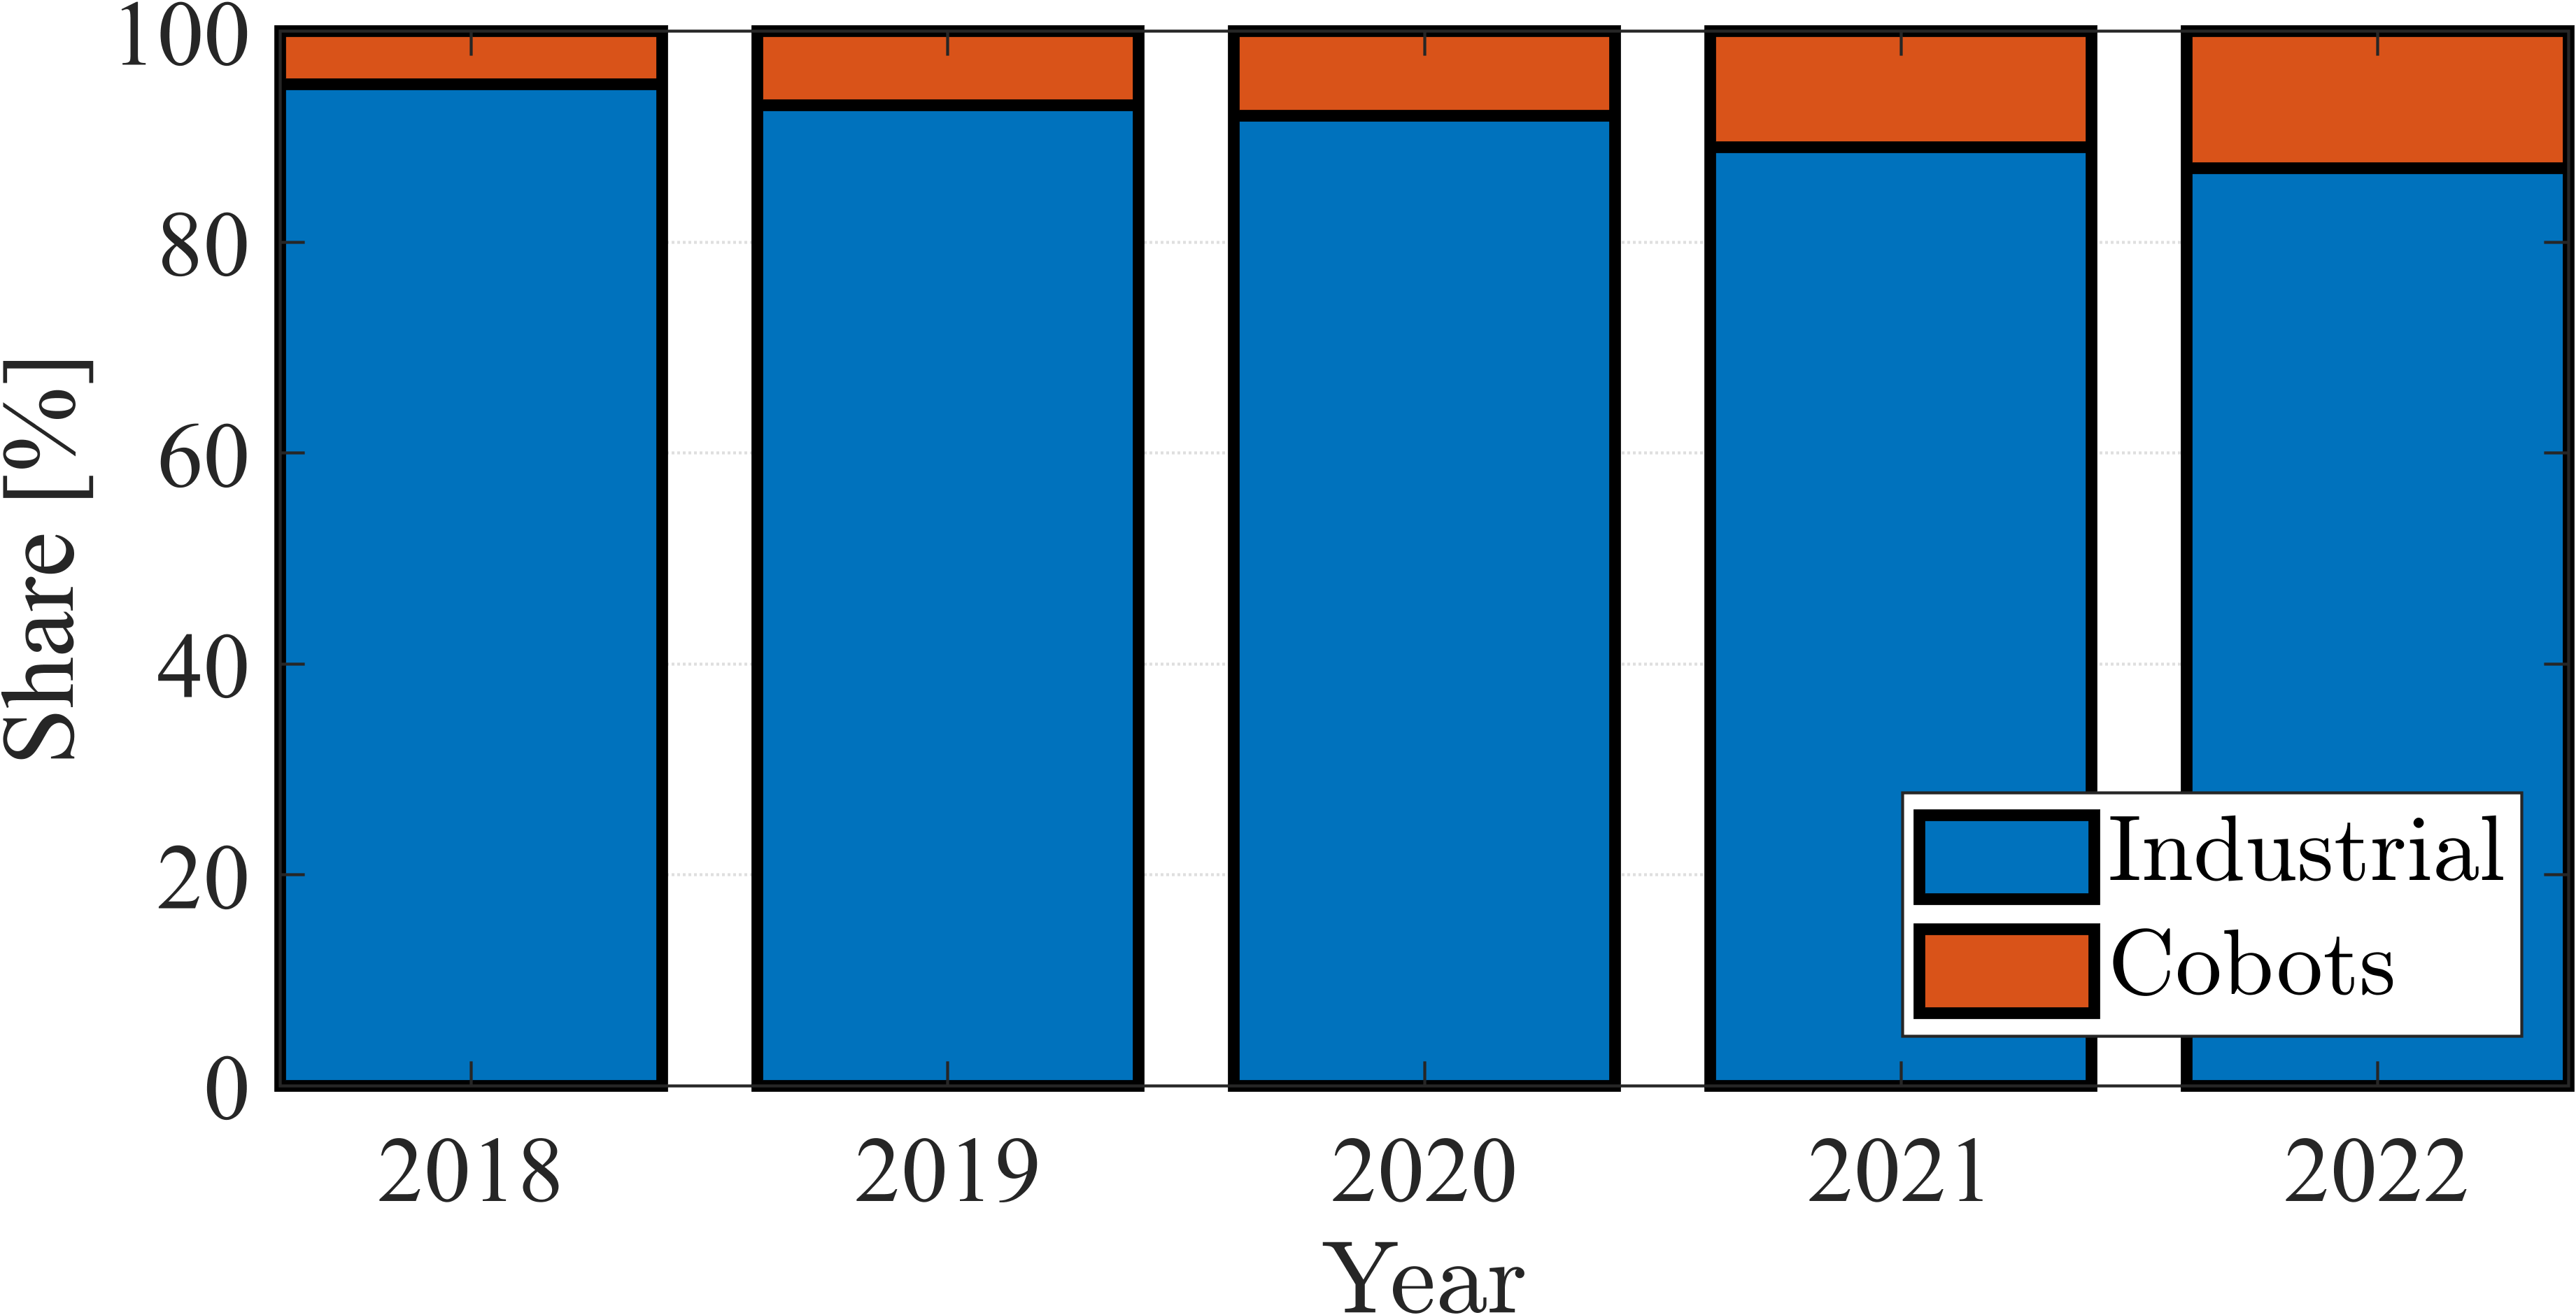
\includegraphics[width= 0.9\columnwidth]{fig/share_industrial_and_cobots} 
	\caption{Ratio of industrial robots to cobots \cite{statista_ir_cobot_share}}
	\label{fig:industrial_cobot_share}
\end{figure}
% ---
% ---------------------------------------------------------------------------------------------------
\subsubsection{Implications}
Modern production paradigms, lifestyle, and societal needs will make robots ubiquitous, permeating many aspects of human life. Consequently, just by their sheer number, industrial, collaborative, and service robots already represent a currently disregarded niche in the global energy landscape. In standard operation, the energy they consume corresponds naturally to the BEE and MI categories in embodied AI systems, and thus, the numbers introduced in this section serve as an indication of the basic energetic requirements in embodied AI. Concretely, the challenge here consists of devising better strategies for efficiently using these legions of robots. If the skills these robots take care of are performed in the most time- and energy-optimal fashion, then BEE and MI energies will also be kept at the optimal minimum.
%---
\begin{figure*}[!t]
	\centering
% 	\hspace*{\fill}
% 	\subfloat[]{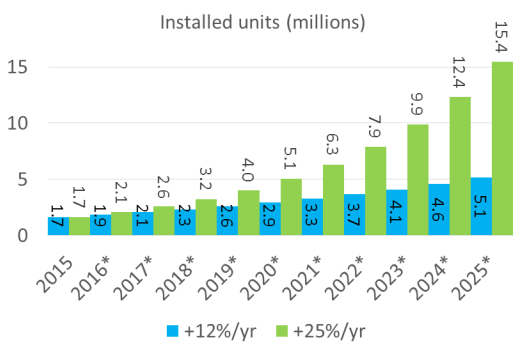
\includegraphics[width= 0.90\columnwidth]{fig/robot_stock} \label{fig:ir_stock}}
% 	\hfill
% 	\subfloat[]{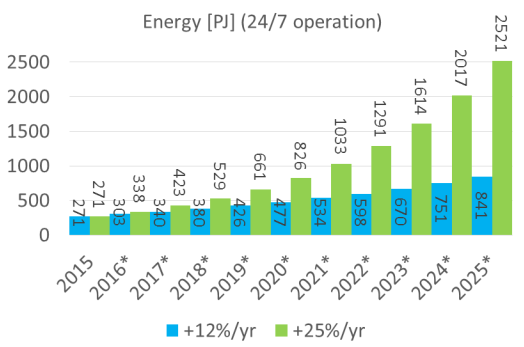
\includegraphics[width= 0.90\columnwidth]{fig/robot_energy} \label{fig:ir_energy}}
% 	\hspace*{\fill}
	\hspace*{\fill}
	\subfloat[]{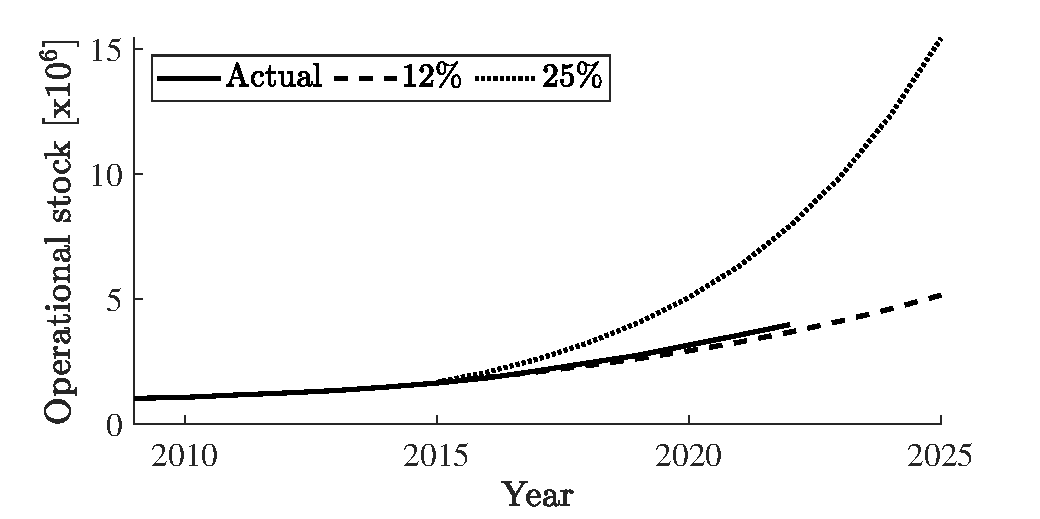
\includegraphics[width= 0.90\columnwidth]{fig/ir_units_projections.pdf} \label{fig:ir_stock}}
	\hfill
	\subfloat[]{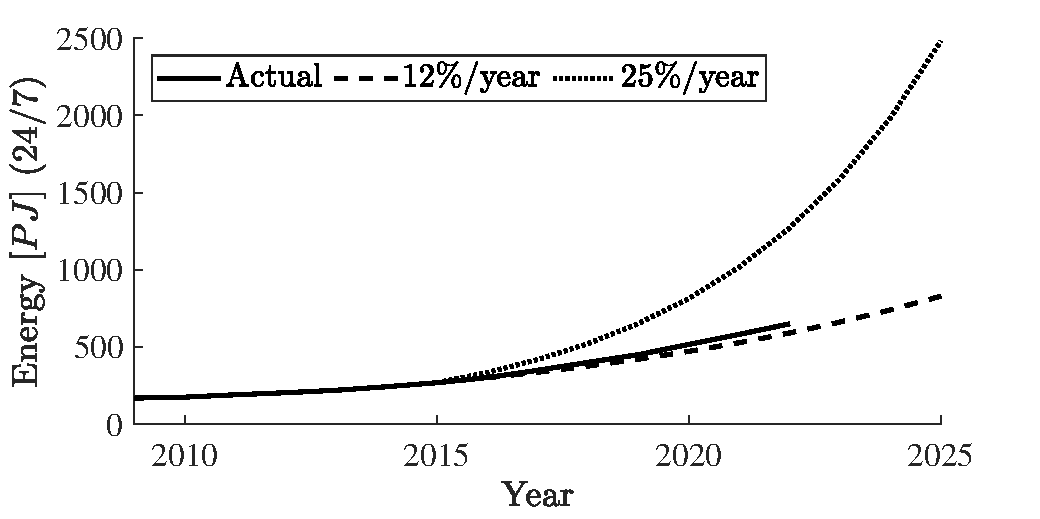
\includegraphics[width= 0.90\columnwidth]{fig/ir_energy_projections.pdf} \label{fig:ir_energy}}
	\hspace*{\fill}
	\\%[-2ex]
	\hspace*{\fill}
	\subfloat[]{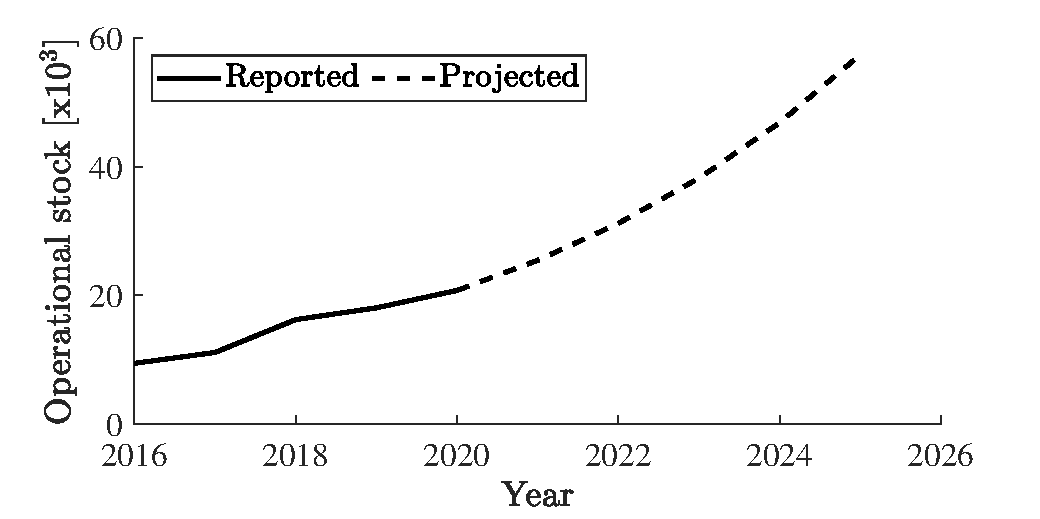
\includegraphics[width= 0.9\columnwidth]{fig/cb_units_projections.pdf}\label{fig:cobot_stock}}
	\hfill    
	\subfloat[]{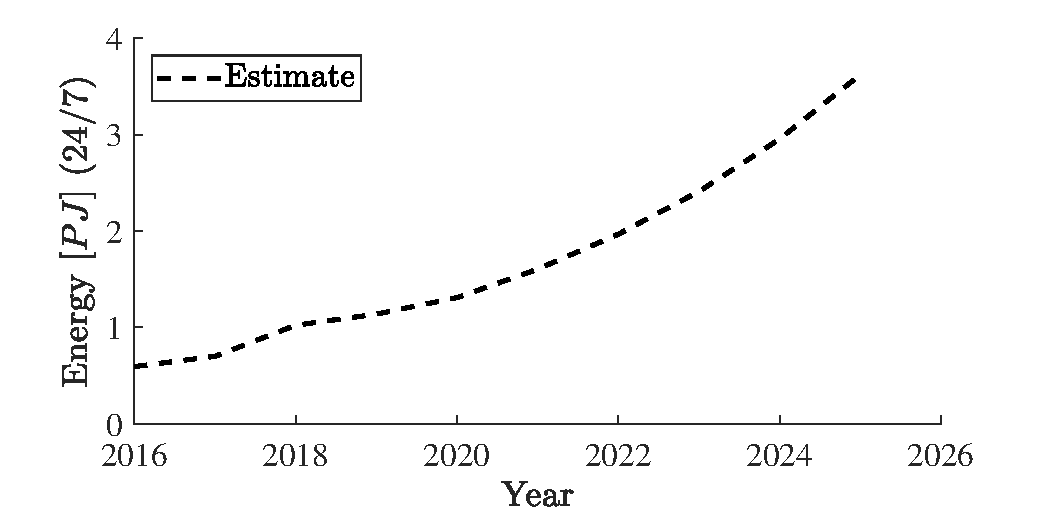
\includegraphics[width= 0.9\columnwidth]{fig/cb_energy_projections.pdf}\label{fig:cobot_energy}}
	\hspace*{\fill}    
	\caption[] {\label{fig:robot_forecasts} Forecasts for robot operational stock reported by the IFR and energy consumption estimates: \subref{fig:ir_stock} industrial robots install base forecast and \subref{fig:ir_energy} estimated worldwide energy consumption, \subref{fig:cobot_stock} cobots install base forecast and their \subref{fig:cobot_energy} estimated worldwide energy consumption.}
\end{figure*}
%---

% SUBSECTION ========================================================================================
\subsection{\textbf{CHALLENGE 3} (C3). Energy for manufacturing}
Although not the focus of this work, we briefly discuss this challenge for completeness and to motivate its study in future works. This last challenge expands the scope and considers the energetic cost of the manufacturing process of the EAI agents. It involves, firstly, the energy to procure the materials needed for manufacturing robots and the computation infrastructure. Secondly, the energy demanded by the manufacturing process itself. As the energy required for material procurement and the manufacturing process is directly linked to the number of EAI agents being manufactured, it can be logically concluded that if their numbers increase exponentially, so will the energy consumed to produce them. Analyzing this demand and devising strategies to handle it are central to this challenge. Although no clear solution is apparent, and since meaningful energy savings in the procurement of raw materials are unrealistic, we see significant potential for energy savings in robot recycling strategies. As a final thought, it is likely that in the future, the manufacturing of EAI agents will be conducted by other EAI agents (e.g., see Fig.~\ref{fig:franka_builds_franka}); thus connecting this challenge directly with the first two challenges.
%---
\begin{figure}[!t]
	\centering
	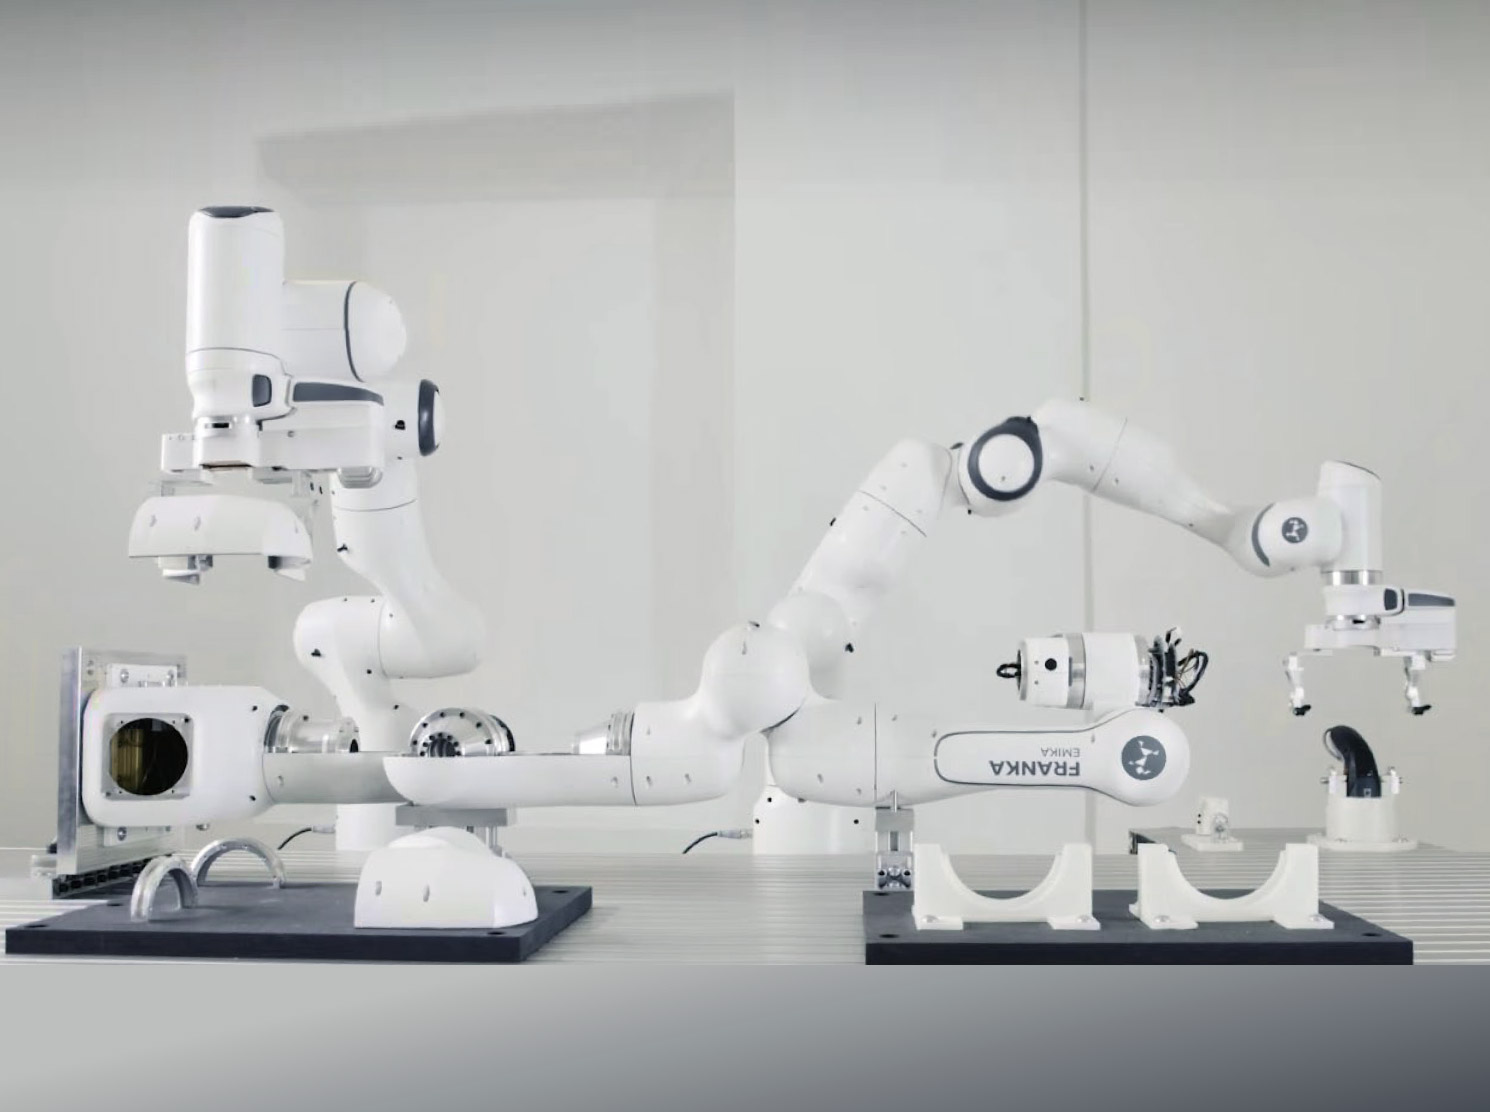
\includegraphics[width=0.75\columnwidth]{fig/franka_builds_franka.jpg}
	\caption{Robots manufacturing more robots}
	\label{fig:franka_builds_franka}
\end{figure}
% ---

% SUBSECTION ========================================================================================
\subsection{Potential research directions}
To identify areas of opportunity given the previously discussed challenges, we first need to consider a crucial fact: for any given task, there is a physical limit to the energy that can be saved. To understand this, consider the following: let $\tau$ be a desired skill for an EAI agent: pick-and-place. Additionally, assume that the optimal trajectory $p$ to move the object from origin to destination is known. Then, the properties of the to-be-moved object and the path $p$ fully determine the minimum energy $E^*_{\tau}$ required to execute skill $\tau$. This means an embodied AI agent attempting to execute $\tau$ will consume at least this much energy. In reality, however, the total energy required for learning and performing a skill comprises the sum of $E^*_{\tau}$ plus the accompanying computational $E_{CCE}$, body-related $E_{BEE}$ and motion and interaction $E_{MIE}$ energy requirements during learning and execution; i.e.
% ---
\begin{equation}
	E_{\tau} =  \underbrace{E^*_{\tau}}_{\text{Skill energy}} + E_{BEE} + \underbrace{E_{CCE} + E_{MIE}}_{\text{Learning energy}}.
\end{equation}
% ---
Fig.~\ref{fig:challengesConnected} depicts the connections between the grand challenges and their associated energy expenditure categories. Related to \textbf{challenge 1} and $E_{CCE}$, one direction that the embodied AI research community should focus on is developing energy-aware algorithms either by concentrating on more data-efficient approaches, embedding relevant prior knowledge in the models or incorporating knowledge sharing capabilities. In particular, the latter would be an ideal candidate solution due to its raw potential. An algorithm capable of sharing and transferring knowledge would allow for high efficiency in multi-skill learning and, associated with a cloud-connected library of skills, would accelerate learning new skills on every EAI agent connected to it. This approach would, over time, convert the processing requirement of the data centers into mostly database storage and query, which is much less energy-demanding.

Additionally, better computational algorithms could be defined, running in more efficient hardware and supported by more efficient communication mechanisms. As for \textbf{challenge 2}, most of the problem links to the rapid growth in the numbers of active robots that will power the future manufacturing industry, but their potential energy-inefficient design and wasted capabilities should not be disregarded. As such, C2 is related to $E_{BEE}$ and $E_{MIE}$. Since there is no control over the eventual number of robots, new designs with lightweight materials and elastic elements that foster the efficient use of the available energy to perform a skill should be pursued. In turn, these new mechatronic designs should be exploited by the embodied AI algorithms researched in \textbf{challenge 1} to find better solutions to learn and execute skills. Finally, \textbf{challenge 3}, is highly intertwined with the first two challenges and, thus, is linked to three types of energy $E_{CCE}$, $E_{BEE}$ and $E_{MIE}$. Consequently, approaches to tackling challenges 1 and 2 will yield improvements in challenge 3. Finally, a parallel and complementary direction to save energy in manufacturing is recycling. A competent recycling process should integrate with manufacturing, where robots can be harvested for materials and parts at the end of their service life.
% ---
\begin{figure}[!t]
	\centering
	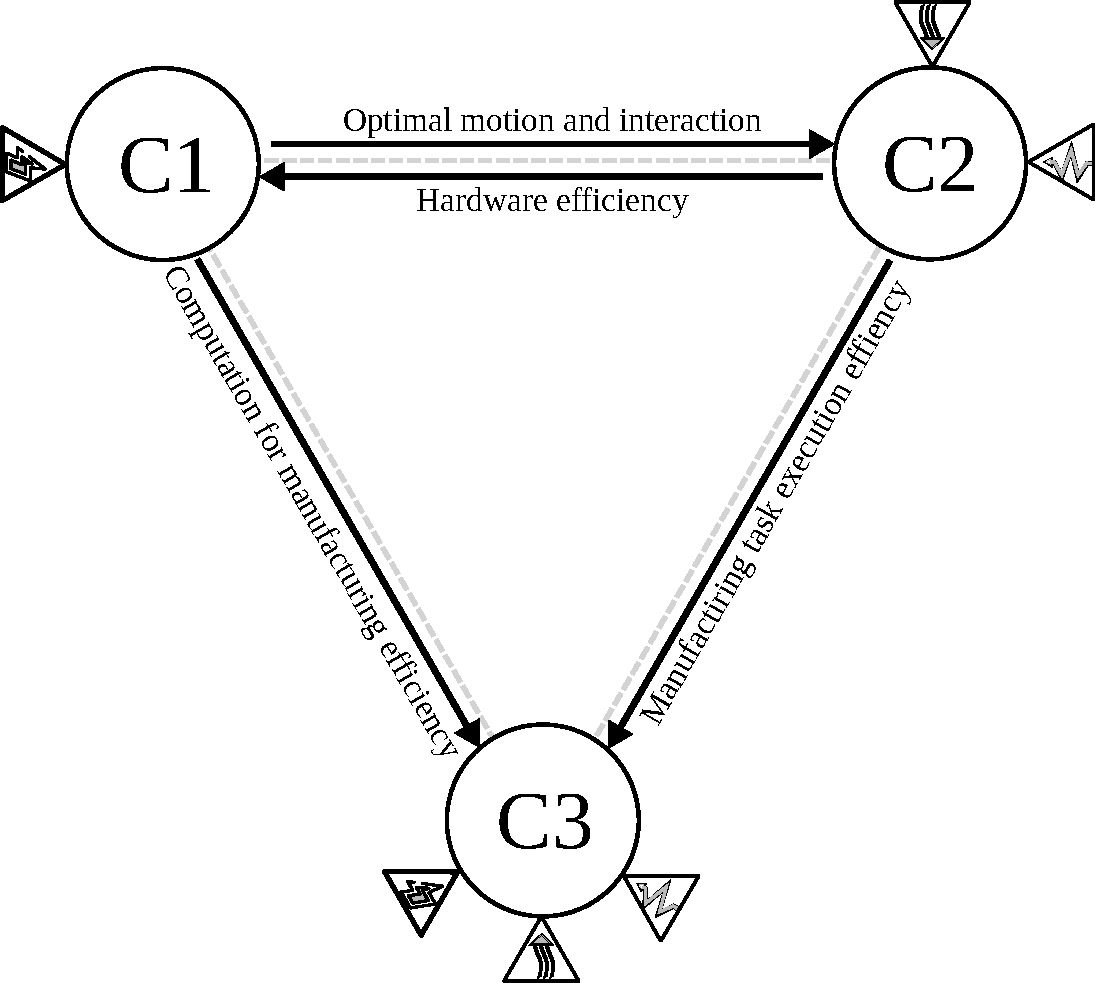
\includegraphics[width=0.8\columnwidth]{fig/grand_challenges_connections.pdf}
	\caption{Interconnection between challenges C1, C2, and C3.}
	\label{fig:challengesConnected}
\end{figure}
% ---